\documentclass[10pt]{article}
\usepackage[french]{babel}
\usepackage[utf8]{inputenc}
\usepackage[T1]{fontenc}
\usepackage{amsmath}
\usepackage{amsfonts}
\usepackage{amssymb}
\usepackage[version=4]{mhchem}
\usepackage{stmaryrd}
\usepackage{graphicx}
\usepackage[export]{adjustbox}
\graphicspath{ {./images/} }

\begin{document}
\section*{Analyse Numérique - correction TD n \({ }^{\circ} \mathbf{2}\) 19-02-2025}
\section*{Exercice 1:}
On sait que \(\gamma\) est l'accélération de la vitesse \(V\) donc

\[
V(t)=V(0)+\int_{0}^{t} \gamma(s) d s \text { et } V(80)=0+\int_{0}^{80} \gamma(s) d s=I
\]

\section*{Par les trapèzes :}
Calculons I par la méthode des trapèzes. Ici, d'après le tableau des valeurs, \(h=10\). On a alors

\[
I=\frac{h}{2}\left(\gamma\left(x_{0}\right)+2 \sum_{i=1}^{n-1} \gamma\left(x_{i}\right)+\gamma\left(x_{n}\right)\right)=\frac{10}{2}(30+2 \times(31,63+\ldots+46,70)+50,67)=3089 m . \mathrm{s}^{-1}
\]

\section*{Par Simpson :}
Calculons I par la méthode de Simpson

\[
\begin{aligned}
V(80) & =\frac{h}{3}\left[\gamma\left(x_{0}\right)+4 \times\left(\gamma\left(x_{1}\right)+\gamma\left(x_{3}\right)+\ldots\right)+2 \times\left(\gamma\left(x_{2}\right)+\gamma\left(x_{4}\right)+\ldots\right)+\gamma\left(x_{n}\right)\right] \\
& =\frac{10}{3}[30+4 \times(31,63+35,47+\ldots)+2 \times(33,44+37,75+\ldots)+50,67]=3087 \mathrm{~m} . \mathrm{s}^{-1}
\end{aligned}
\]

\section*{Exercice 2:}
Soit l'intégrale suivante :

\[
I=\int_{0}^{1} f(x) d x=\int_{0}^{1} 4 \sqrt{1-x^{2}} d x
\]

\begin{enumerate}
  \item Montrer que \(I=\pi\) analytiquement
\end{enumerate}

En faisant le changement de variable suivant

\[
x=\cos y \Rightarrow d x=-\sin y d y
\]

\[
I=\int_{0}^{1} 4 \sqrt{1-x^{2}} d x=\int_{\pi / 2}^{0} 4 \sqrt{1-\cos ^{2} y}(-\sin y d y)
\]

\(I=4 \int_{0}^{\pi / 2}|\sin y| \sin y d y=4 \int_{0}^{\pi / 2} \sin ^{2} y d y=2\left[y-\frac{1}{2} \sin 2 y\right]_{0}^{\pi / 2}=\pi\)\\
2. Donner une approximation du calcul de I en appliquant la méthode de Simpson sur 2 intervalles.

On obtient par la méthode de Simpson par 2 intervalles \([0,1 / 2]\) et \([1 / 2,1]\)\\
\(h=\frac{(1-0)}{2}=\frac{1}{2}\) pour les points d'abscisse \(x_{0}=0, x_{1}=0.5, x_{2}=1.0\)\\
\(I=\frac{\left(x_{1}-x_{0}\right)}{6}\left(f\left(x_{0}\right)+4 f\left(\frac{x_{1}+x_{0}}{2}\right)+f\left(x_{1}\right)\right)+\frac{\left(x_{2}-x_{1}\right)}{6}\left(f\left(x_{1}\right)+4 f\left(\frac{x_{2}+x_{1}}{2}\right)+f\left(x_{2}\right)\right)\)\\
\(I \approx 3,0836\)\\
3. Donner par la méthode de Lagrange, l'expression analytique de la courbe sous laquelle la méthode d'intégration précédente va réellement calculer l'estimation de I et calculer l'aire analytique sous cette courbe.\\
\(y(x)=\frac{(x-0.5)(x-1)}{(-0.5)(-1)} \times 4+\frac{(x)(x-1)}{(0.5)(0.5-1)} \times 3.464+\frac{(x)(x-0.5)}{(1)(1-0.5)} \times 0\)\\
\(\approx-5.856 x^{2}+1.856 x+4\)\\
\(\int_{0}^{1}\left(-5.856 x^{2}+1.856 x+4\right) d x=\left[-5.856 \frac{x^{3}}{3}+1.856 \frac{x^{2}}{2}+4 x\right]_{0}^{1}=2.9760\)

\section*{Exercice 3 :}
1- Calcul exact

La formule de récurrence s'obtient par intégration par parties :\\
\(\left(u(x)=x^{n} ; v^{\prime}(x)=e^{-x}\right)\)\\
\(I_{n}=-e^{-1}+n I_{n-1}\)

En utilisant cette formule de récurrence, en partant de : \(I_{0}=\int_{0}^{1} \exp (-x) d x=1-e^{-1}\), on obtient :\\
\(I_{3}=I=6-16 e^{-1} \approx 0.113928941\)

\section*{Formules de quadrature de type interpolation}
La fonction \(f(x)\) peut être approchée par un polynôme d'interpolation \(P_{n}(x)\) de degré \(n\) ( \(n+1\) points d'interpolation). A l'aide des polynômes de Lagrange \(L_{i}(x)\), la fonction s'écrit de la façon suivante :\\
\(f(x) \approx P_{n}(x)=\sum_{i=0}^{n} y_{i} L_{i}(x)\) avec \(L_{i}(x)=\prod_{\substack{k=0 \\ k \neq i}}^{n} \frac{\left(x-x_{k}\right)}{\left(x_{i}-x_{k}\right)}\) et \(y_{i}=f\left(x_{i}\right)\)\\
D'où\\
\(\int_{a}^{b} f(x) d x \approx \int_{a}^{b} P_{n}(x) d x=\int_{a}^{b} \sum_{i=0}^{n} y_{i} L_{i}(x) d x=\sum_{i=0}^{n} y_{i} \int_{a}^{b} L_{i}(x) d x\)

On pose\\
\(w_{i}=\int_{a}^{b} L_{i}(x) d x\)\\
On a alors la formule suivante\\
\(\int_{a}^{b} f(x) d x \approx \sum_{i=0}^{n} y_{i} w_{i}=\sum_{i=0}^{n} f\left(x_{i}\right) w_{i}\)\\
avec\\
\(f\left(x_{i}\right)=y_{i}\), valeur de la fonction aux points d'interpolation.\\
\(w_{i}=\int_{a}^{b} L_{i}(x) d x\), poids de la formule de quadrature

2- Méthode des trapèzes\\
La méthode des trapèzes correspond à une polynôme d'interpolation de degré \(\mathrm{n}=1\) ( 2 points d'interpolation).\\
Les points d'interpolation sont \(x_{0}=a\) et \(x_{1}=b\)\\
\(\int_{a}^{b} f(x) d x \approx \sum_{i=0}^{1} y_{i} w_{i}=\sum_{i=0}^{1} f\left(x_{i}\right) w_{i}=w_{0} f\left(x_{0}\right)+w_{1} f\left(x_{1}\right)\),\\
\(\int_{a}^{b} f(x) d x \approx w_{0} f(a)+w_{1} f(b)\)\\
avec\\
\(w_{0}=\int_{a}^{b} L_{0}(x) d x=\int_{a}^{b} \frac{\left(x-x_{1}\right)}{\left(x_{0}-x_{1}\right)} d x=\int_{a}^{b} \frac{(x-b)}{(a-b)} d x=\frac{(b-a)}{2}\)\\
\(w_{1}=\int_{a}^{b} L_{1}(x) d x=\int_{a}^{b} \frac{\left(x-x_{0}\right)}{\left(x_{1}-x_{0}\right)} d x=\int_{a}^{b} \frac{(x-a)}{(b-a)} d x=\frac{(b-a)}{2}\)\\
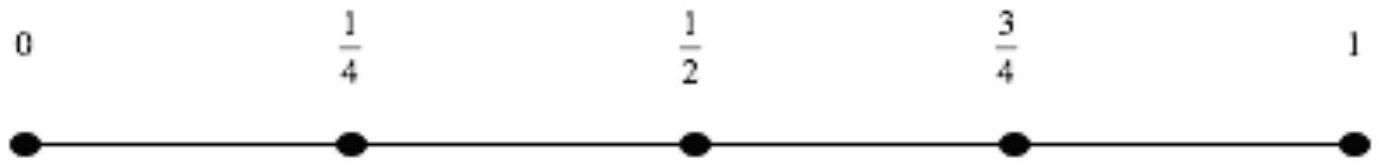
\includegraphics[max width=\textwidth, alt={}, center]{d7843011-bfac-4334-b2db-72b38f93195a-3_165_1379_1382_173}

La méthode de trapèzes sur l'intervalle [a, b] s'écrit\\
\(\int_{a}^{b} f(x) d x \approx w_{0} f(a)+w_{1} f(b)=(b-a) \frac{(f(a)+f(b))}{2}\)

Sur chaque sous-intervalle on applique la méthode des trapèzes et on obtient\\
\(I \approx \frac{1}{4}\left[\frac{f(0)+f\left(\frac{1}{4}\right)}{2}+\frac{f\left(\frac{1}{4}\right)+f\left(\frac{1}{2}\right)}{2}+\frac{f\left(\frac{1}{2}\right)+f\left(\frac{3}{4}\right)}{2}+\frac{f\left(\frac{3}{4}\right)+f(1)}{2}\right]\)\\
\(I \approx \frac{1}{8}\left[f(0)+2 f\left(\frac{1}{4}\right)+2 f\left(\frac{1}{2}\right)+2 f\left(\frac{3}{4}\right)+f(1)\right] \approx 0.1178011137\)

3- Méthode de Simpson\\
La méthode des trapèzes correspond à une polynôme d'interpolation de degré \(\mathrm{n}=2\) ( 3 points d'interpolation).\\
Les points d'interpolation sont \(x_{0}=a, x_{1}=(a+b) / 2\) (point milieu ) et \(x_{2}=b\).

\[
\begin{aligned}
& \int_{a}^{b} f(x) d x \approx \sum_{i=0}^{2} y_{i} w_{i}=\sum_{i=0}^{2} f\left(x_{i}\right) w_{i}=w_{0} f\left(x_{0}\right)+w_{1} f\left(x_{1}\right)+w_{2} f\left(x_{2}\right) \\
& \int_{a}^{b} f(x) d x \approx w_{0} f(a)+w_{1} f\left(\frac{a+b}{2}\right)+w_{2} f(b)
\end{aligned}
\]

Le calcul des poids est le suivant :

\[
\begin{aligned}
& w_{0}=\int_{a}^{b} L_{0}(x) d x=\int_{a}^{b} \frac{\left(x-x_{1}\right)\left(x-x_{2}\right)}{\left(x_{0}-x_{1}\right)\left(x_{0}-x_{2}\right)} d x=\int_{a}^{b} \frac{(x-(a+b) / 2)(x-b)}{(a-(a+b) / 2)(a-b)} d x=\frac{(b-a)}{6} \\
& w_{1}=\int_{a}^{b} L_{1}(x) d x=\int_{a}^{b} \frac{\left(x-x_{0}\right)\left(x-x_{2}\right)}{\left(x_{1}-x_{0}\right)\left(x_{1}-x_{2}\right)} d x=\int_{a}^{b} \frac{(x-a)(x-b)}{((a+b) / 2-a)((a+b) / 2-b)} d x=\frac{4(b-a)}{6} \\
& w_{2}=\int_{a}^{b} L_{2}(x) d x=\int_{a}^{b} \frac{\left(x-x_{0}\right)\left(x-x_{1}\right)}{\left(x_{2}-x_{0}\right)\left(x_{2}-x_{1}\right)} d x=\int_{a}^{b} \frac{(x-a)(x-(a+b) / 2)}{(b-a)(b-(a+b) / 2)} d x=\frac{(b-a)}{6}
\end{aligned}
\]

La méthode de Simpson sur l'intervalle [a, b] s'écrit

\[
\int_{a}^{b} f(x) d x \approx w_{0} f(a)+w_{1} f\left(\frac{a+b}{2}\right)+w_{2} f(b)=\frac{(b-a)}{6}\left[f(a)+4 f\left(\frac{a+b}{2}\right)+f(b)\right]
\]

Sur chaque sous-intervalle on applique la méthode de Simpson et on obtient

\[
I \approx \frac{1}{12}\left[f(0)+4 f\left(\frac{1}{4}\right)+f\left(\frac{1}{2}\right)\right]+\frac{1}{12}\left[f\left(\frac{1}{2}\right)+4 f\left(\frac{3}{4}\right)+f(1)\right] \approx 0.1137754761
\]

4- Quadrature de Gauss

\[
\int_{-1}^{1} f(x) d x \approx \sum_{i=0}^{n} w_{i} f\left(x_{i}\right)
\]

Les 3 racines du polynôme de Legendre \(P_{3}(x)=\frac{1}{2}\left(5 x^{3}-3 x\right)\) sur l'intervalle \([-1,1]\) sont : \(x_{0}=-\sqrt{\frac{3}{5}}, x_{1}=0, x_{2}=\sqrt{\frac{3}{5}}\) avec les poids suivants : \(w_{0}=\frac{5}{9} ; w_{1}=\frac{8}{9} ; w_{2}=\frac{5}{9}\)

Avec ces 3 points, la quadrature de Gauss s'écrit (ici on applique la quadrature sur tout l'intervalle [ \(-1,1\) ])

\[
\int_{-1}^{1} g(x) d x \approx \frac{1}{9}\left[5 g\left(-\sqrt{\frac{3}{5}}\right)+8 g(0)+5 g\left(\sqrt{\frac{3}{5}}\right)\right]
\]

Avant d'appliquer la quadrature, il faut se placer dans l'intervalle \([-1,1]\) en faisant le changement de variables :\\
\(x=\frac{b-a}{2} y+\frac{a+b}{2}\) ce qui entraîne \(d x=\frac{b-a}{2} d y\)\\
\(\int_{a}^{b} f(x) d x=\int_{-1}^{1} \frac{b-a}{2} f\left(\frac{b-a}{2} y+\frac{a+b}{2}\right) d y \approx \sum_{i=0}^{n} w_{i} \frac{b-a}{2} f\left(\frac{b-a}{2} y_{i}+\frac{a+b}{2}\right)\)\\
Posons\\
\(g(y)=\frac{b-a}{2} f\left(\frac{b-a}{2} y+\frac{a+b}{2}\right)\)\\
\(\int_{a}^{b} f(x) d x=\int_{-1}^{1} g(y) d y \approx \sum_{i=0}^{n} w_{i} g\left(y_{i}\right)\)\\
On a alors\\
\(I=\int_{0}^{1} f(x) d x=\int_{0}^{1} x^{3} \exp [-x] d x=\int_{-1}^{1} \frac{1}{2^{4}}(1+y)^{3} \exp \left[-\frac{(1+y)}{2}\right] d y=\int_{-1}^{1} g(y) d y\)\\
avec \(g(y)=\frac{1}{2^{4}}(1+y)^{3} \exp \left[-\frac{(1+y)}{2}\right]\)\\
On a 3 points d'intégration, on obtient\\
\(I=\int_{-1}^{1} g(x) d x \approx w_{0} g\left(x_{0}\right)+w_{1} g\left(x_{1}\right)+w_{2} g\left(x_{2}\right)=\frac{1}{9}\left[5 g\left(-\sqrt{\frac{3}{5}}\right)+8 g(0)+5 g\left(\sqrt{\frac{3}{5}}\right)\right] \approx 0.1139534192\)\\
avec \(g(x)=\frac{1}{2^{4}}(1+x)^{3} \exp \left[-\frac{(1+x)}{2}\right]\)\\
4- Calculer l'erreur relative et absolue\\
Erreurs absolues

\begin{itemize}
  \item Trapèze : 0.00387217273
  \item Simpson : 0.00015346492
  \item Gauss : 0.00002447817
\end{itemize}

Erreurs relatives

\begin{itemize}
  \item Trapèze : 0.03398761277
  \item Simpson : 0.001347023141
  \item Gauss : 0.0002148547137
\end{itemize}

La méthode la plus précise est celle de Gauss, c'est aussi la moins coûteuse car elle ne requiert que 3 évaluations de \(f\), celle du trapèze et de Simpson requièrent 5 évaluations de la fonction.

Exercice 4:\\
Un projectile est lancé avec une vitesse initiale \(\vec{V}_{0}\) à un angle de \(45^{\circ}\). Il est soumis uniquement à la pesanteur.

\begin{enumerate}
  \item En appliquant la relation fondamentale de la dynamique, montrer qu'on obtient un système de deux équations différentielles de deuxième ordre à résoudre :
\end{enumerate}

\[
\left\{\begin{array}{c}
\frac{d^{2} x}{d t^{2}}=0 \\
\frac{d^{2} y}{d t^{2}}=-g
\end{array}\right.
\]

La mécanique du point nous dit qu'il suffit d'appliquer la relation fondamentale de la dynamique au point solide:

\[
m \frac{d \vec{V}}{d t}=\vec{P}=m \vec{g}
\]

Puisqu'il s'agit d'une équation vectorielle, on projette l'équation vectorielle sur les 2 axes \(x\) et \(z\). On arrive donc à un système de deux équations différentielles de deuxième ordre à résoudre.\\
2) Ecrire le système d'équations différentielles sous forme d'un problème de Cauchy.

On pose \(x^{(1)}=v(t)\), l'équation \(\frac{d^{2} x}{d t^{2}}=0\) devient donc le système matriciel suivant:

\[
\frac{d}{d t}\left[\begin{array}{l}
x(t) \\
v(t)
\end{array}\right]=\left[\begin{array}{ll}
0 & 1 \\
0 & 0
\end{array}\right]\left[\begin{array}{l}
x(t) \\
v(t)
\end{array}\right]
\]

On pose \(y^{(1)}(t)=u(t)\), et le système \(\frac{d^{2} y}{d t^{2}}=-g\) devient:\\
\(\frac{d}{d t}\left[\begin{array}{l}y(t) \\ u(t)\end{array}\right]=\left[\begin{array}{ll}0 & 1 \\ 0 & 0\end{array}\right]\left[\begin{array}{l}y(t) \\ u(t)\end{array}\right]+\left[\begin{array}{c}0 \\ -g\end{array}\right]\)\\
On peut regrouper ces deux équations sous la forme d'une seule grande équation matricielle :

\[
\frac{d Y}{d t}=\frac{d}{d t}\left[\begin{array}{c}
x(t) \\
v(t) \\
y(t) \\
u(t)
\end{array}\right]=\left[\begin{array}{llll}
0 & 1 & 0 & 0 \\
0 & 0 & 0 & 0 \\
0 & 0 & 0 & 1 \\
0 & 0 & 0 & 0
\end{array}\right]\left[\begin{array}{c}
x(t) \\
v(t) \\
y(t) \\
u(t)
\end{array}\right]+\left[\begin{array}{c}
0 \\
0 \\
0 \\
-g
\end{array}\right]
\]

ou de manière équivalente sous la forme d'un problème de Cauchy

\[
\frac{d Y}{d t}=f(t, Y(t))=\left[\begin{array}{c}
v(t) \\
0 \\
u(t) \\
-g
\end{array}\right]
\]

avec les conditions initiales

\[
Y_{0}=\left[\begin{array}{l}
x_{0} \\
v_{0} \\
y_{0} \\
u_{0}
\end{array}\right]=\left[\begin{array}{c}
0 \\
V_{0} \cos \left(45^{\circ}\right) \\
0 \\
V_{0} \sin \left(45^{\circ}\right)
\end{array}\right]=\left[\begin{array}{l}
0 \\
1 \\
0 \\
1
\end{array}\right]
\]

\begin{enumerate}
  \setcounter{enumi}{2}
  \item Déterminer sa vitesse et sa position au cours du temps grâce à la méthode d'Euler explicite. On exprimera pour cela le terme général des suites \(\left(x_{n}\right),\left(y_{n}\right),\left(v_{n}\right)\) et \(\left(u_{n}\right)\) correspondant aux composantes suivant \(x\) et \(y\) des vecteurs position et de vitesses respectivement.
\end{enumerate}

Selon la formule d'Euler explicite, on a \(Y_{n+1}=Y_{n}+h f\left(t_{n}, Y_{n}\right)\)\\
\(Y_{n+1}=\left[\begin{array}{c}x_{n+1} \\ v_{n+1} \\ y_{n+1} \\ u_{n+1}\end{array}\right]=\left[\begin{array}{c}x_{n} \\ v_{n} \\ y_{n} \\ u_{n}\end{array}\right]+h\left[\begin{array}{c}v_{n} \\ 0 \\ u_{n} \\ -g\end{array}\right]\)\\
4) Calculer les valeurs des positions et vitesses pour 3 itérations avec :

Les vitesses à l'instant initial \(v_{0}\) et uo sont égales à \(1 \mathrm{~m} / \mathrm{s}\)\\
le pas d'intégration \(h\) est égale \(10^{-4} s\)\\
\(Y_{n+1}=\left[\begin{array}{l}x_{n+1} \\ v_{n+1} \\ y_{n+1} \\ u_{n+1}\end{array}\right]=\left[\begin{array}{l}x_{n} \\ v_{n} \\ y_{n} \\ u_{n}\end{array}\right]+10^{-4}\left[\begin{array}{c}v_{n} \\ 0 \\ u_{n} \\ -9.8\end{array}\right]\)\\
avec \(v_{0}=u_{0}=1 \mathrm{~m} / \mathrm{s}\) avec \(n=0,1,2\)\\
\(Y_{1}=[0.0001 ; 1.0000 ; 0.0001 ; 0.9990]\)\\
\(Y_{2}=[0.0002 ; 1.0000 ; 0.0002 ; 0.9980]\)\\
\(Y_{3}=[0.0003 ; 1.0000 ; 0.0003 ; 0.9971]\)

\section*{Exercice 5 :}
Soit l'équation différentielle ordinaire suivante :

\[
y^{\prime}(t)=f(t, y(t))=1+t^{2}+y(t)
\]

avec la condition initiale \(y_{0}=y(t=0)=1\).

\begin{enumerate}
  \item L'équation discrète en utilisant le schéma d'Euler explicite va s'écrire :
\end{enumerate}

\[
\left\{\begin{array}{l}
y_{n+1}=y_{n}+h\left(1+t_{n}^{2}+y_{n}\right) \\
y_{0}=1
\end{array}\right.
\]

\begin{enumerate}
  \setcounter{enumi}{1}
  \item En utilisant le pas de temps \(h=0.1\), on obtient :
\end{enumerate}

\begin{center}
\begin{tabular}{ccc}
\(n\) & \(t_{n}\) & \(y_{n}\) \\
1 & 0.1 & 1.200 \\
2 & 0.2 & 1.421 \\
\end{tabular}
\end{center}

\begin{enumerate}
  \setcounter{enumi}{2}
  \item En utilisant la méthode d'Euler améliorée, on obtient :
\end{enumerate}

\[
\begin{aligned}
& \left\{\begin{array}{c}
\tilde{y}_{n+1}=y_{n}+h f\left(t_{n}, y_{n}\right) \\
y_{n+1}=y_{n}+h f\left(t_{n+1}, \tilde{y}_{n+1}\right)
\end{array}\right. \\
& \left\{\begin{array}{l}
\tilde{y}_{n+1}=y_{n}+h\left(1+t_{n}^{2}+y_{n}\right) \\
y_{n+1}=y_{n}+h\left(1+t_{n+1}^{2}+\tilde{y}_{n+1}\right)=y_{n}+h\left(1+t_{n+1}^{2}+y_{n}+h\left(1+t_{n}^{2}+y_{n}\right)\right)
\end{array}\right.
\end{aligned}
\]

\begin{enumerate}
  \setcounter{enumi}{3}
  \item Avec le pas \(h=0.1\), on obtient :\\
\(\begin{array}{llll}n & t_{n} & \tilde{y}_{n} & y_{n}\end{array}\)\\
\(\begin{array}{llll}1 & 0.1 & 1.200 & 1.221\end{array}\)\\
\(\begin{array}{llll}2 & 0.2 & 1.444 & 1.469\end{array}\)
\end{enumerate}

\end{document}